\chapter{Fourier series}


%%%%%%%
%
%\section{Notation}
%
%\[\delta_{mn}=\begin{cases}
%                      0   & \mbox{ if }n\neq m\\
%                      1   & \mbox{ if }n=m
%              \end{cases}\]
%%%%%%

\section{The heat equation}

\subsection{What is the heat equation}

The heat equation is a partial differential equation which governs the evolution of a temperature distribution on a one-dimensional rod. If the rod has length $L$ and is parametrised by a coordinate $x\in[0,L]$ and $t$ denotes time then the temperature at time $t$ at position $x$ on the rod is given by a function $\phi(x,t)$. The heat equation is
\[\pd{\phi}{t}=C\ppd{\phi}{x}\]
where $C$ is a constant (we will usually take $C=1$) depending on the material of which the rod is made (how well it conducts and heats up).

\subsection{Where does this equation come from?}

One can derive the heat equation from the following experimentally-observed facts: (a) Heat flows down a temperature gradient. Moreover, it flows at a rate proportional to the gradient $\pd{\phi}{x}$. Let us write $A$ for the constant of proportionality (conductivity). Thus the rate of change of heat energy is $-A\pd{\phi}{x}$ (the minus sign coming from the fact that heat flows {\em down} the gradient). (b) A quantity $\Delta H$ of heat energy will change the temperature of a segment of rod of length $\Delta x$ by $B\Delta H/\Delta x$ where $B$ is a constant (related to the ``specific heat capacity'' of the rod).

Given these two assumptions, if we focus on a small segment of rod between $x$ and $x+\Delta x$ for a short length of time $\Delta t$ then the amount of heat energy which flows in at the point $x$ is approximately $-A\pd{\phi}{x}(x)\Delta t$ and the amount which flows out at $x+\Delta x$ is $-A\pd{\phi}{x}(x+\Delta x)\Delta t$. Thus the total change in heat energy in this segment over the time interval $\Delta t$ is
\[\Delta H=A\Delta t\left(\pd{\phi}{x}(x+\Delta x)-\pd{\phi}{x}(x)\right).\]
This effects a change
\[\Delta\phi=AB\Delta t\frac{\left(\pd{\phi}{x}(x+\Delta x)-\pd{\phi}{x}(x)\right)}{\Delta x}\]
in temperature. Setting $C=AB$, dividing by $\Delta t$ and considering smaller and smaller time intervals and rod segments $\Delta x,\Delta t\to 0$, this expression limits to
\[\pd{\phi}{t}=C\ppd{\phi}{x}.\]

\subsection{How to solve it?}

Let's assume for simplicity that $C=1$ and fix boundary conditions $\phi(0,t)=\phi(\pi,t)=0$. We can spot a few solutions by inspection. For example
\[\phi_1(x,t)=\sin x e^{-t}\]
is a solution (check: $\pd{\phi}{t}=-\sin x e^{-t}$, $\ppd{\phi}{x}=-\sin x e^{-t}$ so $\phi$ satisfies the heat equation). So does
\[\phi_2(x,t)=\sin(2x)e^{-4t}\]
or, more generally,
\[\phi_n(x,t)=\sin(nx)e^{-n^2t}\]
(we'll see later how to get these solutions systematically instead of just guessing them).

Moreover the heat equation is linear: a linear combination of solution is again a solution. Indeed, under suitable convergence assumptions (allowing us to differentiate term-by-term) we can take an infinite linear combination
\[\phi(x,t)=\sum_{n=1}^{\infty}A_n\sin(nx)e^{-n^2t}\]
and the result is still a solution. So we have a vast bank of possible solutions, one for each (suitably convergent) infinite sequence $A_n$.

If we start off with an initial temperature distribution $\phi(x,0)=F(x)$ and fix the boundary conditions as above then we should know the temperature everywhere at all times, so which sequence $A_n$ do we need to pick to get the right solution? Let us substitute the solution into the initial condition:
\[F(x)=\phi(x,0)=\sum_{n=1}^{\infty}A_n\sin(nx)\]
(the $e^{-n^2t}$ terms are all equal to 1 at $t=0$). So the question becomes: given a function $F(x)$, when can we expand it as an infinite linear combination of sine functions? This was the question that Fourier found himself asking after precisely this line of reasoning.

\section{Fourier theory}

Fourier theory provides an expansion of a (more-or-less) arbitrary function $[-L,L]\to\RR$ in terms of sines and cosines.

\begin{thm}
Any sufficiently nice function $F\colon [-L,L]\to\RR$ can be written as a {\emph Fourier series}:
\[F(x)=c+\sum_{n=1}^{\infty}\left(a_n\fcos{n}+b_n\fsin{n}\right).\]
For example, any function on $[-\pi,\pi]$ can be written as
\[F(x)=c+\sum_{n=1}^{\infty}\left(a_n\cos(nx)+b_n\sin(nx)\right).\]
The $a_n,b_n,c$ are called the {\emph Fourier coefficients} of $F$.
\end{thm}

``Sufficiently nice'' could mean, for example, ``differentiable except at a finite collection of points''. When we say ``can be written as'' we mean that the series converges in some sense to the original function. We will not prove this theorem and will defer discussion of convergence till later. Instead, assuming that the theorem is true and that there are no convergence issues, let's work out what the Fourier coefficients would have to be. First we need a lemma.

\begin{lma}
If $n\geq 0$ is an integer then
\begin{align}
\label{eq:fsin}
\int_{-L}^L\fsin{n}dx        &= 0\\
\label{eq:fcos}
\int_{-L}^L\fcos{n}dx        &= 2L\delta_{n0}
\end{align}
If $m,n>0$ are integers then
\begin{align}
\label{eq:fsinfsin}
\int_{-L}^L\fsin{n}\fsin{m}dx&= L\delta_{mn}\\
\label{eq:fcosfcos}
\int_{-L}^L\fcos{n}\fcos{m}dx&= L\delta_{mn}\\
\label{eq:fcosfsin}
\int_{-L}^L\fcos{n}\fsin{m}dx&= 0.
\end{align}
\end{lma}
\begin{proof}[Proof of \eqref{eq:fsinfsin}]
Using the trigonometric identity
\[\cos(A-B)-\cos(A+B)=2\sin(A)\sin(B)\]
we can write the left-hand side of \eqref{eq:fsinfsin} as
\[
\frac{1}{2}\int_{-L}^L\fcos{(n-m)}dx-\frac{1}{2}\int_{-L}^L\fcos{(n+m)}dx
\]
Since we are assuming that $m,n>0$, we have $n+m\neq 0$ so, by \eqref{eq:fcos}, the second integral vanishes. Again, by \eqref{eq:fcos}, the first integral equals $\frac{1}{2}2L\delta_{mn}=L\delta_{mn}$.
\end{proof}

Using these formulae, we can find $c$, $a_n$ and $b_n$:

\begin{thm}\label{thm:fouco}
If
\[F(x)=c+\sum_{n=1}^{\infty}\left(a_n\fcos{n}+b_n\fsin{n}\right)\]
then
\begin{align}
\label{eq:fourierc}
   c   &    = \frac{1}{2L}\int_{-L}^LF(x)dx\\
\label{eq:fourierA}
   a_m &    = \frac{1}{L}\int_{-L}^LF(x)\fcos{m}dx\\
\label{eq:fourierB}
   b_m &    = \frac{1}{L}\int_{-L}^LF(x)\fsin{m}dx
\end{align}
\end{thm}
\begin{proof}[Proof of \eqref{eq:fourierc}]
\begin{align*}
 \int_{-L}^LF(x)dx
        & = \int_{-L}^{L}cdx
            + \sum_{n=1}^{\infty}\int_{-}^La_n\fcos{n}\\
&\qquad\qquad+ \sum_{n=1}^{\infty}\int_{-}^Lb_n\fsin{n}\\
        & = 2Lc
            + 0
            + 0
\end{align*}

so $c=\frac{1}{2L}\int_{-L}^LF(x)dx$.
\end{proof}
\begin{proof}[Proof of \eqref{eq:fourierA}]
\begin{align*}
 \int_{-L}^LF(x)\fcos{m}dx
        & = \int_{-L}^{L}c\fcos{m}dx
            + \sum_{n=1}^{\infty}\int_{-}^La_n\fcos{n}\fcos{m}\\
&\qquad\qquad+ \sum_{n=1}^{\infty}\int_{-}^Lb_n\fsin{n}\fcos{m}\\
        & = 0
            + L\sum_{n=1}^{\infty}\delta_{mn}a_n
            + 0\\
        & = La_m
\end{align*}

so

\[
  a_m = \frac{1}{L}\int_{-L}^LF(x)\fcos{m}dx
\]
\end{proof}

The proof of \eqref{eq:fourierB} is left as an exercise.

\begin{exm}\label{exm:fxequalsx}
Consider the function $F(x)=x$ on the interval $[-\pi,\pi]$ (i.e. $L=\pi$). Its Fourier coefficients are given by
\begin{align*}
c&=\frac{1}{2\pi}\int_{-\pi}^{\pi}xdx\\
&=\frac{1}{2\pi}\left[\frac{x^2}{2}\right]_{-\pi}^{\pi}\\
&=0\\
a_n&=\frac{1}{\pi}\int_{-\pi}^{\pi}x\cos nx dx\\
&=\frac{1}{\pi}\left(\left[x\frac{\sin(nx)}{n}\right]_{-\pi}^{\pi}-\int_{-\pi}^{\pi}\frac{\sin(nx)}{n}\right)\\
&=0+\frac{1}{n^2\pi}\left[\cos(nx)\right]_{-\pi}^{\pi}\\
&=0
\end{align*}
(where we have used $\sin(\pm\pi)=0$ and $\cos(n\pi)=\cos(-n\pi)$) and
\begin{align*}
b_n&=\frac{1}{\pi}\int_{-\pi}^{\pi}x\sin nx dx\\
&=\frac{1}{\pi}\left(\left[-x\frac{\cos(nx)}{n}\right]_{-\pi}^{\pi}+\int_{-\pi}^{\pi}\frac{\cos(nx)}{n}\right)\\
&=(-\cos(n\pi)/n-\cos(n\pi)/n)+\frac{1}{n^2\pi}\left[\sin(nx)\right]_{-\pi}^{\pi}\\
&=-2\cos(n\pi)/n\\
&=2(-1)^{n+1}/n
\end{align*}
where we have used that $\cos(n\pi)=(-1)^n$.

Therefore the Fourier series of $F(x)=x$ on $[-\pi,\pi]$ is
\[x=2\sum_{n=1}^{\infty}\frac{(-1)^{n+1}}{n}\sin(nx),\]
that is
\[x=2\left(\frac{\sin(x)}{1}-\frac{\sin(2x)}{2}+\frac{\sin(3x)}{3}-\cdots\right)\]
We should think of this as an infinite series of approximations to $x$, obtained by truncating the sum after finitely many terms. We plot the graphs of these truncations in Figure \ref{fig:fourier-x} below and you can see that the graphs are tending (in some fairly weak sense) to the graph of the straight line.
\end{exm}

\begin{figure}
\label{fig:fourier-x}
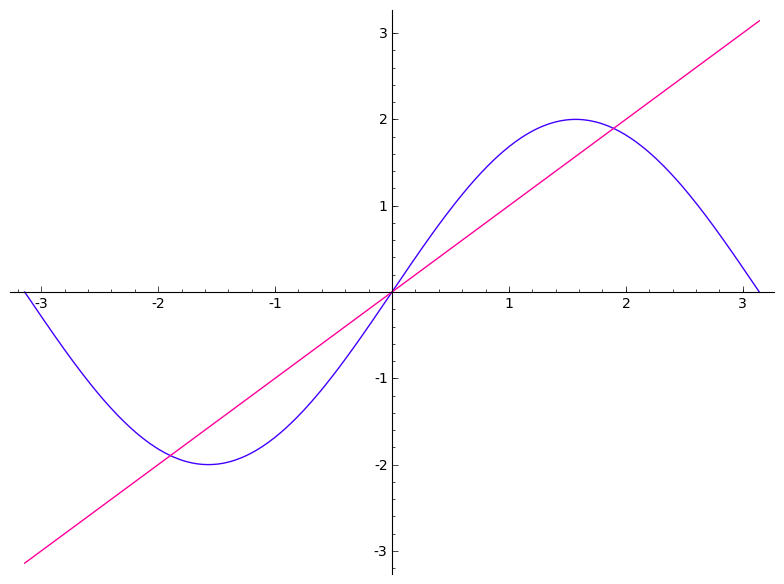
\includegraphics[width=200px]{fourier-1.png}
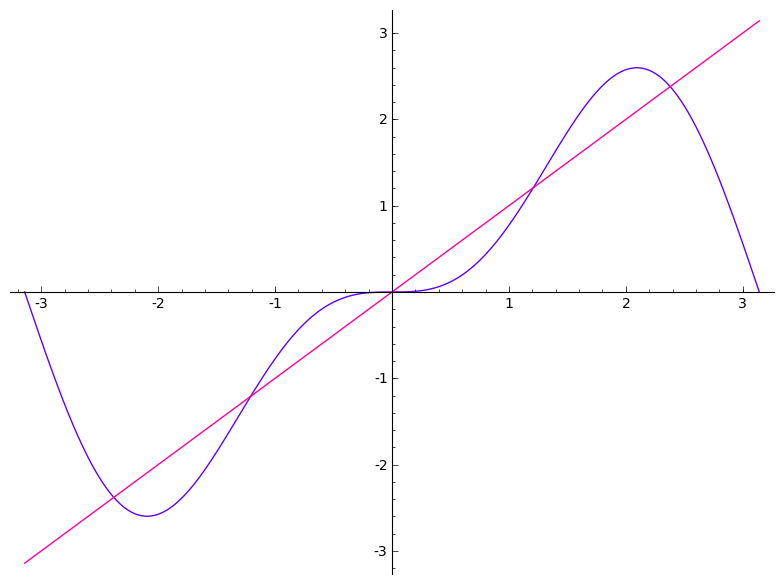
\includegraphics[width=200px]{fourier-2.png}
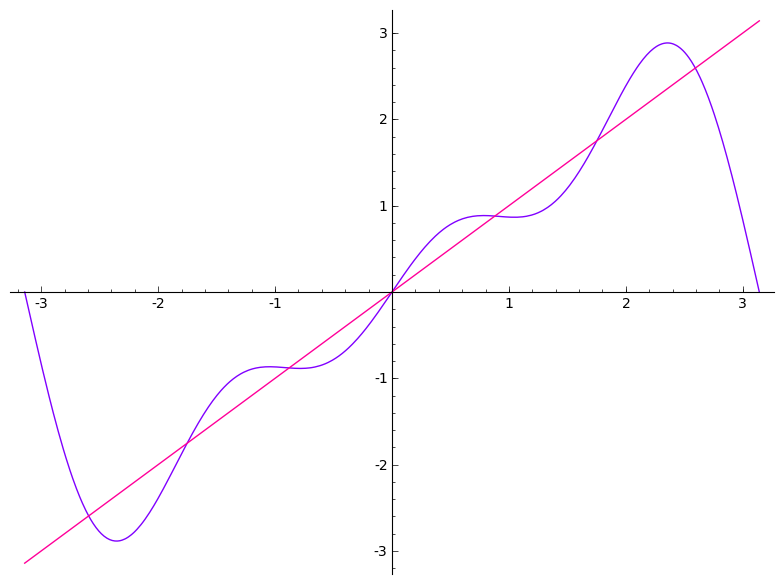
\includegraphics[width=200px]{fourier-3.png}
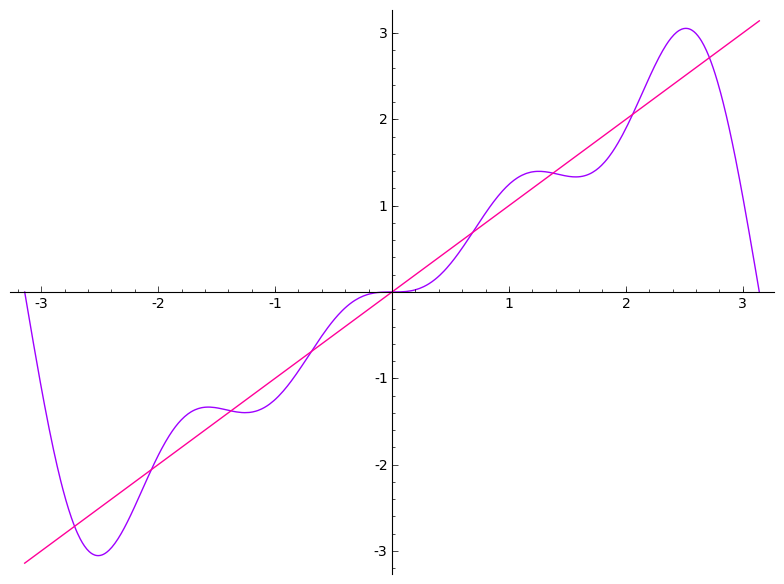
\includegraphics[width=200px]{fourier-4.png}
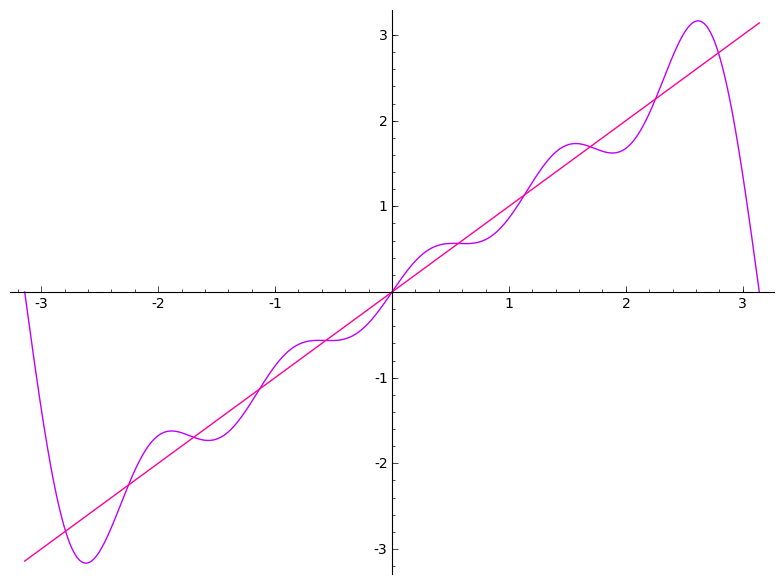
\includegraphics[width=200px]{fourier-5.png}
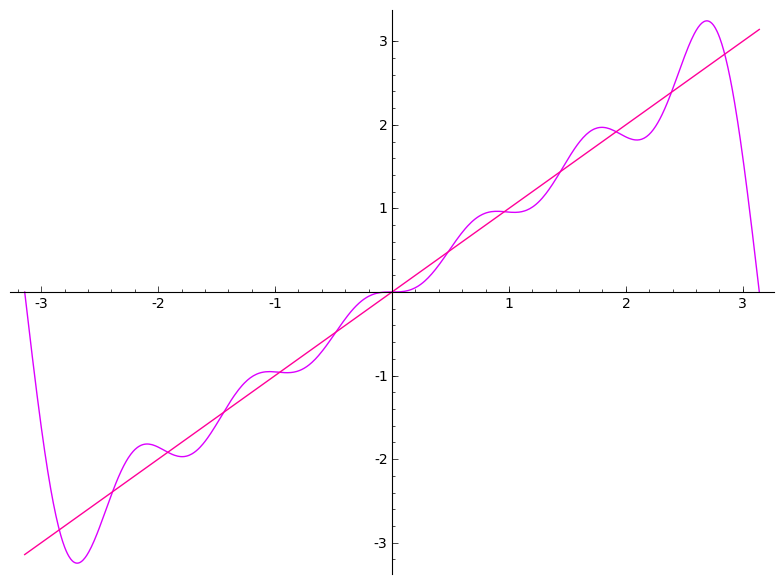
\includegraphics[width=200px]{fourier-6.png}
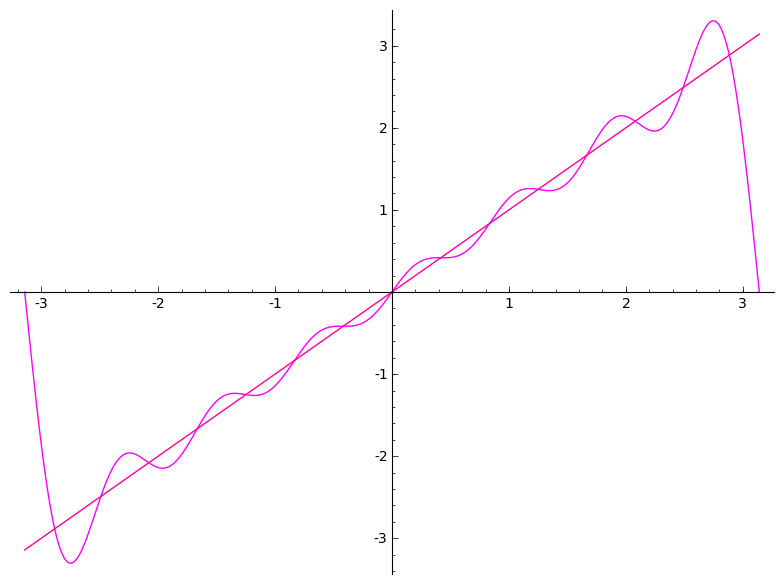
\includegraphics[width=200px]{fourier-7.png}
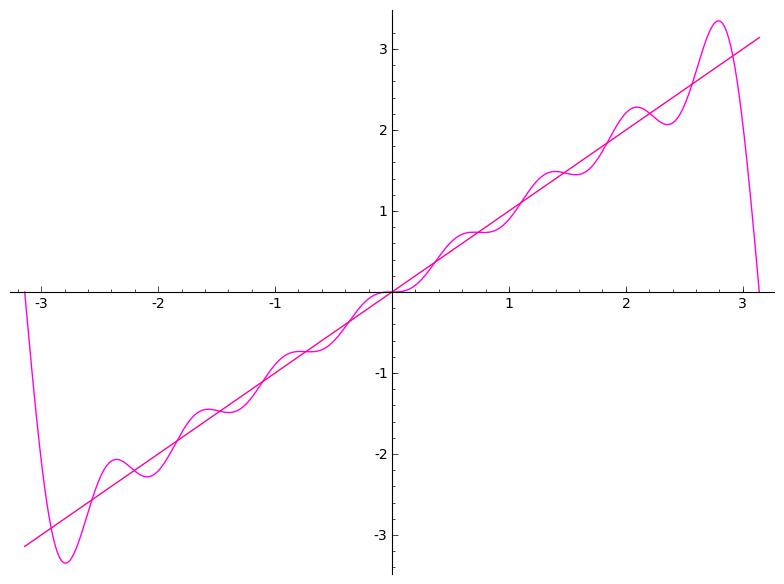
\includegraphics[width=200px]{fourier-8.png}
\caption{The graphs of $2\sum_{n=1}^N\frac{(-1)^{n+1}}{n}\sin(nx)$ for $N=1,2,3,4,5,6,7,8$.}
\end{figure}

Notice that there is a shortcut to computing Fourier series when the function has certain symmetries. A function $F$ is {\em odd} if $F(-x)=-F(x)$ and {\em even} if $F(-x)=F(x)$ (so $F(x)=x$ is odd and $F(x)=\cos(x)$ is even).
\begin{lma}
Suppose $F$ has Fourier series.
\[F(x)=c+\sum_{n=1}^{\infty}\left(a_n\fcos{n}+b_n\fsin{n}\right)\]
If $F$ is even then:
\begin{itemize}
\item $b_n=0$,
\item $a_n=\frac{2}{L}\int_0^LF(x)\fcos{n}dx$,
\item $c=\frac{1}{L}\int_0^LF(x)dx$.
\end{itemize}
If $F$ is odd then:
\begin{itemize}
\item $b_n=\frac{2}{L}\int_0^LF(x)\fsin{n}dx$,
\item $a_n=0$,
\item $c=0$.
\end{itemize}
\end{lma}
We saw this in the previous example: $F(x)=x$ is odd and we found $a_n=c=0$.
\begin{proof}[Proof of Lemma]
Let us show that $F(x)$ even implies $b_n=0$ (the other proofs proceed in exactly the same way).

We have
\begin{align*}
b_n&=\frac{1}{L}\int_{-L}^LF(x)\fsin{n}dx\\
   &=\frac{1}{L}\left(\int_{-L}^0F(x)\fsin{n}dx+\int_0^LF(x)\fsin{n}dx\right)
\end{align*}
(that is we split the range of the integral in half and perform each half separately). Substituting $u=-x$ in the first integral gives
\[\int_{-L}^0F(x)\fsin{n}dx=\int_{L}^0F(-u)\sin\left(\frac{-n\pi u}{L}\right)(-du)\]
using $F(-u)=F(u)$ (evenness) and $\sin(-n\pi u/L)=-\sin(n\pi u/L)$ we get
\[\int_L^0F(u)\sin\left(\frac{n\pi u}{L}\right)du\]
or
\[-\int_0^LF(u)\sin\left(\frac{n\pi u}{L}\right)du\]
(swapping the limits of the integral swaps the sign). Therefore
\[b_n=-\int_0^LF(u)\sin\left(\frac{n\pi u}{L}\right)du+\int_0^LF(x)\sin\left(\frac{n\pi x}{L}\right)dx=0\]
as required.
\end{proof}

\begin{exm}
Consider ($L=1$)
\[F(x)=\begin{cases}0&\mbox{ if }x\in[-1,0)\\ \tfrac{1}{2}&\mbox{ if }x=0\\1&\mbox{ if }x\in(0,1].\end{cases}\]
This function is neither odd nor even, but if we subtract $1/2$ then we get an odd function
\[G(x)=\begin{cases}-\tfrac{1}{2}&\mbox{ if }x\in[-1,0)\\ 0&\mbox{ if }x=0\\\tfrac{1}{2}&\mbox{ if }x\in(0,1].\end{cases}\]
This has Fourier coefficients
\begin{align*}
b_n&=2\int_0^1G(x)\sin(n\pi x)dx\\
   &=\int_0^1\sin(n\pi x)dx\\
   &=\frac{1}{n\pi}[-\cos(n\pi x)]_0^1\\
   &=\frac{1-(-1)^n}{n\pi}.
\end{align*}
That means that $b_n=2/n\pi$ if $n$ is odd and zero if $n$ is even. Therefore $G(x)=\frac{2}{\pi}\sin(\pi x)+\frac{2}{3\pi}\sin(3\pi x)+\cdots$ and
\[F(x)=\frac{1}{2}+\frac{2}{\pi}\sin(\pi x)+\frac{2}{3\pi}\sin(3\pi x)+\cdots\]
\end{exm}

\begin{exm}\label{exm:fxequalsxsquared}
Consider $F(x)=x^2$ on the interval $[-\pi,\pi]$. This function is even so $b_n=0$ automatically. We have
\[c=\frac{1}{\pi}\int_0^{\pi}x^2dx=\frac{\pi^3}{3}\]
and
\begin{align*}
a_n&=\frac{2}{\pi}\int_0^{\pi}x^2\cos(nx)dx\\
   &=\frac{2}{\pi}\left(\cancelto{0}{\left[x^2\frac{\sin(nx)}{n}\right]_0^{\pi}}-\frac{2}{n}\int_0^{\pi}x\sin(nx)dx\right)\\
   &=-\frac{4}{n\pi}\left(\left[-x\frac{\cos(nx)}{n}\right]_0^{\pi}+\frac{1}{n}\int_0^{\pi}\cos(nx)dx\right)\\
   &=\frac{4}{n^2}(-1)^n-\cancelto{0}{\frac{1}{n}\left[-\frac{\sin(nx)}{n}\right]_0^{\pi}}\\
   &=\frac{4(-1)^n}{n^2}
\end{align*}
therefore
\[x^2=\frac{\pi^2}{3}-4\left(\cos x-\frac{\cos 2x}{4}+\frac{\cos 3x}{9}-\cdots\right)\]
on $[-\pi,\pi]$.
\end{exm}

\subsection{Half-range Fourier series}

Often we only specify the values of a function on the interval $[0,L]$ and we only want to see sine terms in its Fourier expansion (we will see this when we solve the heat equation).

\begin{dfn}
Suppose that $F(x)$ is a function $[0,L]\to\RR$. Define its {\em odd extension} to be the function
\[F_{even}(x)=\begin{cases}F(x)&\mbox{ if }x>0\\ -F(-x)&\mbox{ if }x<0.\end{cases}\]
The half-range sine series of $F$ is then defined to be the Fourier series of $F_{even}$, in other words
\[F(x)=\sum_{n=1}^{\infty}b_n\fsin{n}\]
on $[0,L]$ where $b_n=\frac{2}{L}\int_0^LF(x)\fsin{n}dx$.
\end{dfn}
Analogously one can define the half-range cosine series by taking the Fourier series of the even extension
\[F_{odd}(x)=\begin{cases}F(x)&\mbox{ if }x>0\\ F(-x)&\mbox{ if }x<0.\end{cases}\]

\begin{exm}\label{exm:xpiminusxsquared}
Consider the function $F(x)=x(\pi-x)$ on the interval $[0,\pi]$. We have
\begin{align*}
b_n&=\frac{2}{\pi}\int_0^{\pi}x(\pi-x)\sin(nx)dx\\
   &=\frac{2}{\pi}\left(\cancelto{0}{\left[-x(\pi-x)\frac{\cos(nx)}{n}\right]_0^{\pi}}+\frac{1}{n}\int_0^{\pi}(\pi-2x)\cos(nx)dx\right)\\
   &=\frac{2}{n\pi}\left(\left[(\pi-2x)\frac{\sin(nx)}{n}\right]_0^{\pi}+\frac{1}{n}\int_0^{\pi}2\sin(nx)dx\right)\\
   &\frac{4((-1)^{n+1}+1)}{n^3\pi}\\
   &=\begin{cases}
       \frac{8}{n^3\pi}&\mbox{ if }n\mbox{ is odd}\\
       0&\mbox{ if }n\mbox{ is even}
     \end{cases}
\end{align*}
so
\[x(\pi-x)=8\left(\frac{\sin x}{\pi}\sin x+\frac{\sin 2x}{8\pi}+\frac{\sin 3x}{27\pi}+\cdots\right)\]
on $[0,\pi]$. Note that in this example, although the function $x(\pi-x)$ is not odd (or even!), we are taking its odd extension and computing the Fourier series of that which is why only sine terms appear. This is what we call the half-range sine series.
\end{exm}

\section{Parseval's theorem}

\begin{thm}[Parseval's theorem]
If $F(x)=c+\sum_{n=1}^{\infty}\left(a_n\fcos{n}+b_n\fsin{n}\right)$ then
\[\frac{1}{L}\int_{-L}^LF(x)^2dx=2c^2+\sum_{n=1}^{\infty}(a^2_n+b^2_n).\]
\end{thm}
\begin{proof}
We have:
\begin{align*}
\frac{1}{L}\int_{-L}^LF(x)^2dx&=\frac{1}{L}\int_{-L}^LF(x)\left(c+\sum_{n=1}^{\infty}\left(a_n\fcos{n}+b_n\fsin{n}\right)\right)dx\\
     &=\frac{c}{L}\int_{-L}^LF(x)dx+\sum_{n=1}^{\infty}\frac{a_n}{L}\int_{-L}^LF(x)\fcos{n}dx+\sum_{n=1}^{\infty}\frac{b_n}{L}\int_{-L}^LF(x)\fsin{n}dx\\
&=2c^2+\sum_{n=1}^{\infty}(a^2_n+b^2_n)
\end{align*}
using the formulae for $c,a_n,b_n$ given in Theorem \ref{thm:fouco}.
\end{proof}

\begin{cor}
We have
\[\frac{\pi^2}{6}=\sum_{n=1}^{\infty}\frac{1}{n^2}.\]
\end{cor}
\begin{proof}
Take $F(x)=x$ on $[-\pi,\pi]$. We computed the Fourier series of $F(x)$ on $[-\pi,\pi]$ in Example \ref{exm:fxequalsx} and found
\[F(x)=\sum_{n=1}^{\infty}\frac{2(-1)^{n+1}}{n}\sin(nx).\]
Applying Parseval's theorem implies that
\[\frac{1}{\pi}\int_{-\pi}^{\pi}x^2dx=\sum_{n=1}^{\infty}\frac{4}{n^2}\]
and the left-hand side equals $2\pi^2/3$. Rearranging gives the desired relationship.
\end{proof}

\begin{cor}
We have
\[\frac{\pi^4}{90}=\sum_{n=1}^{\infty}\frac{1}{n^4}.\]
\end{cor}
\begin{proof}
Take $F(x)=x^2$ on $[-\pi,\pi]$. We computed the Fourier series of $F(x)$ on $[-\pi,\pi]$ in Example \ref{exm:fxequalsxsquared} and found
\[F(x)=\frac{\pi^2}{3}+\sum_{n=1}^{\infty}\frac{4(-1)^n}{n^2}\cos(nx).\]
Applying Parseval's theorem implies that
\[\frac{1}{\pi}\int_{-\pi}^{\pi}x^4dx=\frac{2\pi^4}{9}+\sum_{n=1}^{\infty}\frac{16}{n^4}\]
The left-hand side equals $\frac{2\pi^4}{5}$ so rearranging gives
\[\frac{\pi^4}{90}=\frac{1}{16}\left(\frac{2\pi^4}{5}-\frac{2\pi^4}{9}\right)=\sum_{n=1}^{\infty}\frac{1}{n^4}\]
as required.
\end{proof}

In general, when it converges, the sum $\zeta(s):=\sum_{n=1}^{\infty}\frac{1}{n^s}$ is called the {\em Riemann zeta function} so we have evaluated $\zeta(2)=\frac{\pi^2}{6}$ and $\zeta(4)=\frac{\pi^4}{90}$.

\section{The Hilbert space picture}

\subsection{An analogy}

Parseval's theorem says that
\[F(x)=c+\sum_{n=1}^{\infty}\left(a_n\fcos{n}+b_n\fsin{n}\right)\]
implies
\[\frac{1}{L}\int_{-L}^LF(x)^2dx=2c^2+\sum_{n=1}^{\infty}(a^2_n+b^2_n).\]
This looks a little bit like Pythagoras's theorem, which says that
\[v=ae_1+be_2\]
implies that
\[|v|^2=a^2+b^2.\]
Here $e_1$ and $e_2$ are an orthonormal basis for $\RR^2$ and $|v|^2$ denotes the squared length of the vector $v$.

To make this analogy precise, we should consider $F$ as a vector in a vector space. Which vector space? The vector space of real-valued functions on $[-L,L]$! You can add functions, you can multiply them by real numbers and they obey the axioms (e.g. distributivity) required to form a vector space.

Then we should think of $1$ (the constant function), $\fcos{n}$ and $\fsin{n}$ as basis vectors in this space of functions. When we write $F$ as a Fourier series we are expanding in terms of this basis. Notice that in the definition of ``basis'' we are only allowed to take finite linear combinations of basis vectors, so Fourier series are something more general. We say that $1,\fcos{n},\fsin{n}$ form a {\em Hilbert space basis} for the space of functions.

Notice that since our basis consists of infinitely many (linearly independent) functions, our vector space must be infinite-dimensional.

We should also think of $\frac{1}{L}\int_{-L}^LF(x)^2dx$ as the ``length'' of the vector $F$. Indeed we will think of
\[\left\langle F,G\right\rangle:=\frac{1}{L}\int_{-L}^LF(x)G(x)dx\]
as a ``dot product'' (or {\em inner product}) between functions $F$ and $G$ thought of as vectors in the vector space of functions. With respect to this inner product, the basis vectors $1$, $\fcos{n}$ and $\fsin{n}$ satisfy orthogonality relations
\begin{align*}
\left\langle \fsin{n},\fcos{m}\right\rangle&=\frac{1}{L}\int_{-L}^L\fsin{n}\fcos{m}dx=0\\
\left\langle \fsin{n},1\right\rangle&=\frac{1}{L}\int_{-L}^L\fsin{n}=0\\
\left\langle \fcos{n},1\right\rangle&=\frac{1}{L}\int_{-L}^L\fcos{n}=0\\
\left\langle \fsin{n},\fsin{m}\right\rangle&=\frac{1}{L}\int_{-L}^L\fsin{n}\fsin{m}dx=\delta_{mn}\\
\left\langle \cos{n},\fcos{m}\right\rangle&=\frac{1}{L}\int_{-L}^L\fcos{n}\fcos{m}dx=\delta_{mn}\\
\left\langle 1,1\right\rangle&=\frac{1}{L}\int_{-L}^Ldx=2
\end{align*}
by the Fourier integral identities! This makes it {\em almost} an orthonormal basis - the only problem being that $1$ has length $2$. Normalising this we get a unit vector $1/\sqrt{2}$. This accounts for the random factor of 2 that crops up in Parseval's theorem in front of $c^2$.

In general a (real\footnote{There are also complex Hilbert spaces.}) {\em Hilbert space} is a vector space over $\RR$ with an inner product satisfying:
\begin{itemize}
\item $\langle x,y\rangle=\langle y,x\rangle$,
\item $\langle ax+by,z\rangle=a\langle x,z\rangle+b\langle y,z\rangle$,
\item $\|x\|^2:=\langle x,x\rangle\geq 0$ with equality if and only if $x=0$,
\item the space is {\em complete} in the following sense. Suppose that $v_k$ is a sequence of vectors such that $\sum_{k=1}^N\|v_k\|^2<\infty$. Then there exists a vector $v$ such that
\[\left\|v-\sum_{k=1}^{N}v_k\right\|\to 0\]
as $N\to\infty$.
\end{itemize}
This final axiom is the important one. It allows us to make sense of infinite sums like Fourier series.

\subsection{A word about convergence}

Note that $\left\langle F,F\right\rangle$ only makes sense if $F^2$ is integrable. So we should restrict to functions for which $\int_{-L}^LF(x)^2dx$ exists and is finite. These are called $L^2$-functions and the inner product $\left\langle,\right\rangle$ is called the $L^2$-inner product ($\left\langle F,F\right\rangle$ is called the $L^2$-norm of $F$). We often write $\|F\|^2=\left\langle F,F\right\rangle$.

The convergence of a Fourier series to $F$ is to be understood in the $L^2$ sense, that is if $F_N=c+\sum_{n=1}^N\left(a_n\fcos{n}+b_n\fsin{n}\right)$ then
\[\|F-F_N\|^2\to 0\mbox{ as }N\to\infty.\]
This is a relatively weak notion of convergence. It means that the squared difference between the function and its $N$th Fourier approximation is small {\em on average} (but not necessarily small everywhere). This is known as a least-squares approximation. There are certainly examples where, for some $x$, $F_N(x_0)$ does not converge to $F(x_0)$ as $N\to\infty$. This happens for example at a discontinuity of $F$ (see the pictures of the Fourier series of $F(x)=x$ on $[-\pi,\pi]$, for example - you can think of this as having a discontinuity at $\pm\pi$ because if you wrap back around then the function jumps down from $\pi$ to $-\pi$). The least-squares convergence means that the region in which the function is poorly-approximated gets smaller and smaller as $N$ increases.

For some functions (e.g. differentiable functions) the Fourier series does converge pointwise everywhere (i.e. $F_N(x_0)\to F(x_0)$ for all $x_0$). Here differentiability is understood to mean that even if we extend $F$ periodically to the whole of $\RR$ by setting $F(x+2nL)=F(x)$, then the result is differentiable (this is not the case for $F(x)=x$).



\iffalse
\section{Examples}

\begin{exm}[The saw-tooth wave]
The function $G(x)=x$ is not $2L$-periodic. However, there is a $2L$-periodic function $F(x)=x-2L[x/2L]-L$ which agrees with $G(x)$ on $[-L,L]$. It is easier t imagine its graph: take the graph of $G(x)=x$ on $[-L,L]$ and translate it to live over $\ldots,[-5L,-3L],[-3L,-L],[-L,L],[L,3L],[3L,5L],\ldots$ to get a ``saw-tooth wave''. We will now compute the Fourier coefficients of $F(x)$.

\begin{align*}
  c  & = \int_{-L}^Lxdx\\
     & = \left[\frac{x^2}{2}\right]_{-L}^L\\
     & = 0
\end{align*}

\begin{align*}
  A_n &=
\end{align*}
\end{exm}



In fact, {\emph any} function $G$ whose domain of definition includes the interval $[-L,L]$ can be used to generate a $2L$-periodic function $F(x)=G(x-2L[x/2L]-L)$ which agrees with $G$ on the interval $[-L,L]$. The moral of this is: whenever I take the Fourier expansion of a function $G$ which seems not to be periodic (like $G(x)=x$ or $G(x)=x^2$) I am really taking the Fourier expansion of the unique periodic function which agrees with $G$ on $[-L,L]$.

\begin{exm}[The square wave]
The function $G(x)=\begin{cases}0&\mbox{ if }x<0\\ 1&\mbox{ if }x\geq 1\end{cases}$ gives a $2L$-periodic function $F(x)=G(x-2L[x/2L]-L)$ whose graph looks like a ``square wave''.
\end{exm}

\fi